The PC environment had morphed significantly between the development of Wolfenstein 3D in 1991 and the development of \doom{} in 1993. The previous "recommended configuration" based on an Intel 386 with 2~MiB of RAM and a VGA graphics card was no more.\\
\par
The "new" top of the line PC still had six subsystems: \circled{1}~Inputs, \circled{2}~Bus, \circled{3}~CPU, \circled{4}~RAM, \circled{5}~Video~output, and \circled{6}~Audio~output together forming a pipeline. Each of them had become faster or increased in capacity.\\
\par
\vspace{2mm}
\drawing{pc_components}{The six components of an IBM PC.}
\par
 Before describing each component in detail, an important clarification is required. Since this chapter is structured as a delta comparing what was available for \doom{} to what was available for Wolfenstein 3D, it carries a feeling of abounding power which is deceiving. \\
 \par
 Despite the impressive list of improvements listed next, keep in mind that the IBM PCs were still not machines well suited for video games. They were riddled with limitations due to the original target, which was office work. They were designed to perform word processing, crunch spreadsheets and maybe occasionally display a static graph -- the intent was never to build something allowing real time, 70Hz\footnote{VGA's most common refresh rate used for games (320x200) was 70Hz, contrary to today's ubiquitous 60Hz.} animations.\\ 
\par 
Looking back it is hard to believe that studios focused solely on producing titles for a machine "obviously" less capable than consoles. The list of problems was substantial:
\begin{itemize}
\item A CPU unable to perform floating-point operations and no co-processors.
\item An archaic graphics system seemingly unable to double-buffer and with an aspect ratio different from the monitor, resulting in distorted images.
\item A de-facto sound system only capable of irritating "beeps" and a fragmented sound card ecosystem when the customer had elected to buy one.
\item A price tag where a top of the line machine fetched close to \$3,000. To compare with the competition, the SNES and the SEGA Genesis were both priced at US\$199 while the Neo-Geo which provided arcade-like experience was priced at US\$649.99\footnote{Adjusted for inflation the figure would be, as of 2018: \$10,476 for a PC, \$377.00 for a SNES/Genesis, and \$1,134 for a Neo-Geo.}.
\end{itemize}
\par
 A PC was unappealing at best and seemingly less likely to generate good games, especially compared to cheaper systems which had been built with 60Hz animation in mind and benefited from sprite engines.\\
 \par
  Obviously, given the title of the book in your hands, with a few software tricks the hardware of the PC was capable of far more than what it was designed for. PCs were not good at certain types of games but they could excel at certain types requiring a framebuffer. In a world without Internet and little documentation, it was far from a trivial challenge.\\
\par

Figure ~\ref{ibm_ps1_top} on the opposite page reproduces the kind of advertisement one could find in abundance in the many computer magazines of the 90s. Notice the featured IBM PS/1 with an Intel 486 CPU emphasizes office work and its ability to run static-screened office applications. Productivity and profit were the only way to justify the high price of a machine that represented 5\% of the US median yearly income in 1993\footnote{ "statista.com" lists 1993 US median income at \$52,335. Byte Magazine's Spring 1993 ads show 486 DX2-66 VESA PCs at \$2,575.}.\\
\par

 % (\$2,000\footnote{\$13,000 in 2017.}). Also worth mentioning, the "huge" standard 14" CRT which must have weighted close to 20 pounds!\\
\par
\begin{figure}[H] \centering
\fullimage{ibm_ps1_top}
\caption{IBM PS/1 ad circa 1993. Notice the ridiculously small 14" CRT standard monitor allowing a resolution up to 800x600.}
\label{ibm_ps1_top}
\end{figure}


















\cleartoleftpage
 
\cfullimage{PX486P3/b-486-px486p3_romain}{Motherboard PX486P3 by QDI Computer, Inc.}
A practical way to get an overview of the hardware available is to open up a PC and take a look at the component that connects everything together. In 1994, the best-selling motherboard was the PX486P3 by QDI Computer, Inc\footnote{A Canadian company \scaledimage{0.03}{Canada} !}.\\

\par
The most prominent novelty is of course the heart of the computer, the Intel i486 CPU \circled{1}. A closer look reveals many more features which would turn out to be of paramount importance for the architecture of \doom.\\
\par 
The black connectors show the traditional ISA bus expansion ports. One 8-bit \circled{2} and three dual-slot 16-bit \circled{3} allow four ISA cards. Also present are three connectors of a new kind with an additional brown slot \circled{4}. These are VLB slots\footnote{a.k.a: VL-Bus, a.k.a: VESA Local Bus.}, a bus up to 10x faster than ISA.

\drawing{px486p3}{Component diagram of the PX486P3.}
\par
In the upper left \circled{6}, the main memory of the system had grown in capacity, speed and complexity. Thanks to a sharp decline in manufacturing price, the standard DRAM\footnote{Dynamic RAM.} installed would be 4 MiB\footnote{\doom{} would not run on PCs equipped with only 2 MiB.}.\\
\par
 Finally, in the upper right \circled{5}, a new type of RAM had found its way into these new PCs. Eight black chips of SRAM\footnote{Static RAM.} offered a total of 256 KiB acting as L2 "cache". Used in a new system designed to prevent CPU data and instruction starvation, the SRAM was much faster (access time of 20ns, which was 10x faster than DRAM) but had the double drawbacks of being far more expensive to produce and being less dense than DRAM, limiting its usability.



% \begin{enumerate}
% \item RAM prices had dropped significantly. The standard 2 MiB was not a whooping 4 MiB. 
% \item Bandwidth hungry GUI and had lead motherboard manufacturers to come up with a faster bus called VLB.
% \item The sound generator ecosystems was even more fragmented than before with more and more manufacturer producing sound cards.
% \item Not visible on the drawing, the operating system shortcomings were being addressed by independent developers via something called "DOS eXtenders".
% \item Unsurprisingly the impossible to program VGA was still the standard but manufacturers were now competing to produce the faster DACs and \fixme{"RAMDAC"}?.
% \item CACHE
% \end{enumerate}
\pagebreak
\trivia{Several of the most impressive game studios of the era speculated on the projected RAM price drop. The most impressive titles of 1994 (including \doom) required a minimum of 4 MiB installed. Strike Commander, Ultima 8, and Comanche Maximum Overkill are prime examples.
\par
\begin{center}
\scaledimage{0.32}{box_strike_commander.png}  \scaledimage{0.32}{box_ultima8.png} \scaledimage{0.32}{box_comanche.png}
\end{center}
}
Ironically this time period would end up coinciding with the great RAM shortage of 1994 which saw the price go back up. The legend attributes the surge to a resin factory burning down in Taiwan. In all likelihood the fluctuation was probably due to Microsoft's announcement of Windows 95, which recommended a machine with at least 8 MiB of RAM.

\begin{center}
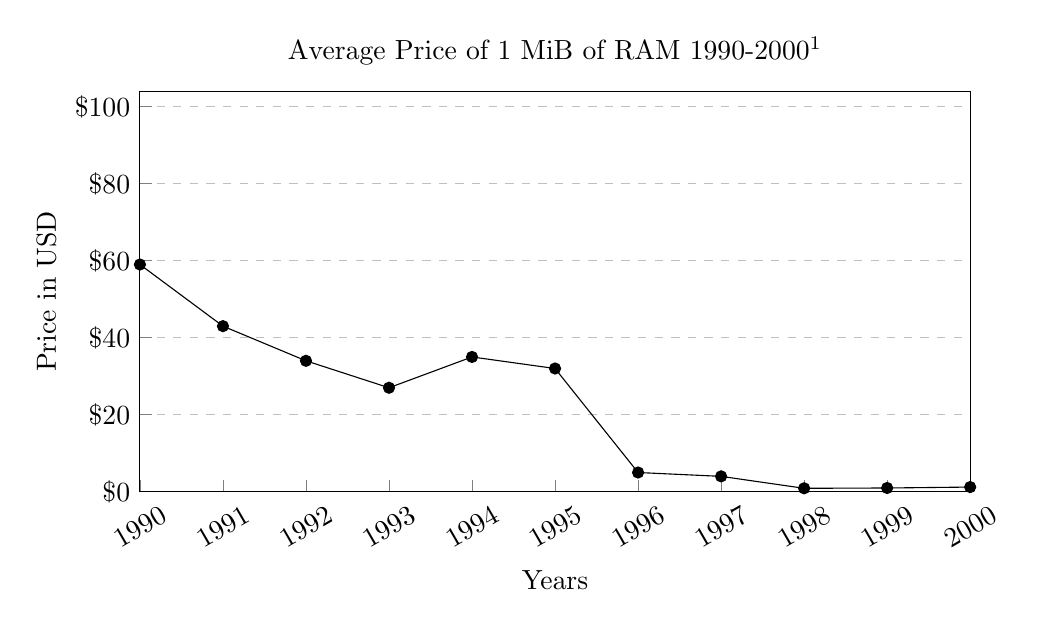
\begin{tikzpicture}

\begin{axis}[
    width=1.0\textwidth,
    height=0.55\textwidth,
    title={Average Price of 1 MiB of RAM 1990-2000\protect\footnotemark},
    xlabel={Years},
    xtick pos=left,
    ytick pos=left,
    ylabel={Price in USD},
    yticklabel={${\$\pgfmathprintnumber{\tick}}$},
    xticklabel style={ rotate=30,},
    xticklabel style={/pgf/number format/1000 sep=},
    xmin=1990, xmax=2000,
    ymin=0, ymax=104,
    %xtick={0,20,40,60,80,100},
    %ytick={0,20,40,60,80,100,120},
    legend pos=north west,
    ymajorgrids=true,
    grid style=dashed,
]
 
\addplot[
    color=black,
    mark=*,
    ]
    coordinates {
    (1990,59)
      (1991,43)
      (1992,34)
      (1993,27)
      (1994,35)
    (1995,32)
      (1996,5)
      (1997,4)
      (1998,0.9)
      (1999,0.98)
      (2000,1.22)
    
    };
 
\end{axis}
\end{tikzpicture}
\end{center}
\footnotetext{Source: John C. McCallum survey.}





